\documentclass[11pt,a4paper,oneside]{report}

\usepackage{style/manuel_style}

% --- Metadonnees ---
\newcommand{\manuelversion}{1.0}
\newcommand{\manueldate}{Mai 2026}

\begin{document}

% =====================================================================
%  PAGE DE GARDE
% =====================================================================
\begin{titlepage}
    \begin{tikzpicture}[remember picture, overlay]
        % Bandeau supérieur
        \fill[aifoilprimary] (current page.north west)
            rectangle ([yshift=-4cm]current page.north east);
        % Bandeau inférieur
        \fill[aifoilrule] (current page.south west)
            rectangle ([yshift=2cm]current page.south east);
    \end{tikzpicture}

    \vspace*{1cm}
    \begin{flushright}
        \color{white}
        \fontfamily{phv}\selectfont
        \textbf{\fontsize{42}{50}\selectfont AifoilTools}\\[6pt]
        {\fontsize{18}{22}\selectfont Analyse aérodynamique 2D}\\
        {\fontsize{18}{22}\selectfont de profils d'aile}
    \end{flushright}

    \vfill

    \begin{center}
        \color{aifoilprimary}
        \fontfamily{phv}\selectfont
        \textbf{\Huge Manuel utilisateur}\\[1em]
        {\Large Version \manuelversion{} --- \manueldate}
    \end{center}

    \vfill

    \begin{flushleft}
        \color{white}
        \fontfamily{phv}\selectfont
        \large
        \textbf{Nervures}\\
        Conception assistée par ordinateur de parapentes
    \end{flushleft}
    \vspace{0.5cm}
\end{titlepage}

% =====================================================================
%  CREDITS / LICENCE
% =====================================================================
\thispagestyle{empty}
\null
\vfill
\begin{flushleft}
    \small
    \textbf{AifoilTools --- Manuel utilisateur, version \manuelversion}\\
    Édition de \manueldate.\\[1em]

    Ce document décrit l'utilisation de la bibliothèque
    \textbf{AifoilTools} et de son interface graphique pour
    l'analyse aérodynamique 2D de profils d'aile par couplage avec
    le solveur \emph{XFoil}.\\[0.5em]

    AifoilTools est distribué sous licence \textbf{LGPL-3.0}.
    Le code source est disponible à l'adresse :\\
    \url{https://github.com/BenoitGFree/AifoilTools}\\[0.5em]

    \emph{XFoil} est un logiciel développé par Mark Drela (MIT) et
    distribué sous licence GPL.\\[0.5em]

    Toutes les marques citées sont la propriété de leurs détenteurs
    respectifs.
\end{flushleft}
\clearpage

% =====================================================================
%  TABLE DES MATIERES
% =====================================================================
\pagenumbering{roman}
\tableofcontents
\clearpage
\listoffigures
\clearpage

\pagenumbering{arabic}

% =====================================================================
%  CHAPITRES
% =====================================================================
\chapter{Présentation}
\label{chap:introduction}

\section{À propos d'AirfoilTools}

\textbf{AirfoilTools} est une bibliothèque Python d'outils dédiés
à l'analyse aérodynamique 2D de profils d'aile. Elle a été extraite
du projet \emph{Axile} (logiciel de conception de parapentes
développé par Nervures) afin de constituer une boîte à outils
réutilisable pour des applications variées : voile, parapente,
hélices, ailes d'avions modèles réduits, etc.

L'application combine :

\begin{itemize}
    \item un \textbf{moteur géométrique} fondé sur les courbes de
        Bézier de degré arbitraire et les splines multi-segment
        (BezierSpline) avec continuités paramétrables (C\textsuperscript{0},
        C\textsuperscript{1}, C\textsuperscript{2}) ;
    \item un \textbf{couplage avec XFoil}, le solveur
        aérodynamique de référence pour les écoulements 2D
        subsoniques visqueux ;
    \item une \textbf{interface graphique interactive} permettant
        l'édition des profils, le pilotage des simulations et la
        visualisation comparative des résultats.
\end{itemize}

\screenshot{01_main_window.png}{1.0}{%
    Vue générale de l'application au démarrage : profils
    NACA~2412 (courant, en bleu) et NACA~0012 (référence,
    en rouge).}

\section{À qui s'adresse ce manuel}

Ce manuel s'adresse aux \textbf{utilisateurs} de l'application
graphique. Il couvre l'ensemble des fonctionnalités accessibles
depuis l'interface, depuis le chargement d'un profil jusqu'à
l'analyse comparative des polaires aérodynamiques.

Les développeurs intéressés par l'API Python de la bibliothèque
trouveront la documentation technique dans le code source
(docstrings au format Sphinx) et dans la documentation générée
(dossier \chemin{docs/}).

\begin{noteinfo}
Aucune connaissance préalable en aérodynamique théorique
n'est requise pour utiliser l'application. En revanche, une
compréhension générale des grandeurs aérodynamiques (coefficient
de portance $C_L$, de traînée $C_D$, finesse $C_L/C_D$,
nombre de Reynolds, angle d'incidence $\alpha$) facilite
l'interprétation des résultats.
\end{noteinfo}

\section{Architecture fonctionnelle}

L'application est structurée autour de \textbf{trois onglets}
correspondant à autant d'étapes logiques :

\begin{enumerate}
    \item \menu{Profils} --- chargement, édition et comparaison des
        profils géométriques. Deux profils sont gérés simultanément :
        un \emph{profil courant} (en bleu) modifiable, et un
        \emph{profil de référence} (en rouge) qui sert de
        comparaison.
    \item \menu{Paramétrage XFoil} --- saisie des paramètres de
        simulation : plage de Reynolds, balayage en incidence,
        paramètres de couche limite, options de panneaux.
    \item \menu{Résultats} --- présentation graphique des résultats
        sous forme de \emph{grille configurable de cellules
        d'analyse}, chacune affichant un tracé indépendant
        (polaire $C_L(\alpha)$, $C_D(\alpha)$, finesse, distribution
        de pression $-C_p(x)$, profil de couche limite, etc.).
\end{enumerate}

\section{Représentation des profils}

AirfoilTools propose deux modes de représentation des profils :

\subsection*{Mode points discrets}

Le profil est défini par une suite de points dans la convention
\textbf{Selig} (parcours du bord de fuite vers l'extrados, puis
le bord d'attaque, puis l'intrados, et retour au bord de fuite).
C'est le format le plus courant des bibliothèques de profils
(par exemple \chemin{airfoiltools.com}).

\subsection*{Mode spline (Bézier multi-segment)}

Le profil est défini par deux \textbf{BezierSpline} (extrados et
intrados), composées chacune de plusieurs segments de Bézier
raccordés en continuité C\textsuperscript{1}. Ce mode permet :

\begin{itemize}
    \item une \emph{édition interactive} par déplacement des
        points de contrôle ;
    \item un \emph{ré-échantillonnage à la demande} avec une
        densité de points librement choisie ;
    \item le \emph{calcul exact de la courbure et des tangentes}
        en tout point ;
    \item le \emph{split d'un segment} en deux à un point arbitraire
        (algorithme de De Casteljau, mathématiquement exact).
\end{itemize}

Le passage d'un mode à l'autre se fait via le menu
\menu{Édition $\rightarrow$ Convertir en Spline} ou par chargement
d'un fichier au format \chemin{.bspl} ou \chemin{.bez}.

\begin{astuce}
Pour bénéficier pleinement des fonctionnalités d'édition
interactive et du tracé de la courbure, il est recommandé
de \textbf{convertir vos profils en mode Spline} dès le
chargement. Les chapitres suivants détaillent cette procédure.
\end{astuce}

\chapter{Installation et lancement}
\label{chap:installation}

\section{Prérequis}

\begin{itemize}
    \item \textbf{Système d'exploitation} : Windows 10 ou 11
        (testé), Linux et macOS (compatibilité a priori, non
        testée par les développeurs).
    \item \textbf{Python} : version 3.10 ou supérieure
        (recommandation : 3.13).
    \item \textbf{Solveur XFoil} : nécessaire uniquement pour
        l'exécution des simulations. Sous Windows, l'exécutable
        \chemin{xfoil.exe} est fourni dans le dossier
        \chemin{externaltools/xfoil/} de la distribution.
\end{itemize}

\section{Distribution exécutable Windows}

Pour les utilisateurs Windows ne souhaitant pas installer Python,
une distribution \chemin{.exe} autonome est disponible. Elle
intègre l'interpréteur Python, l'ensemble des dépendances et le
binaire XFoil.

L'application se lance en double-cliquant sur
\chemin{AifoilTools.exe}.

\begin{noteinfo}
Au premier lancement, Windows peut afficher un avertissement
\emph{SmartScreen} car l'exécutable n'est pas signé. Cliquez
sur \og Informations complémentaires \fg{} puis \og Exécuter
quand même \fg{} pour autoriser le lancement.
\end{noteinfo}

\section{Installation depuis les sources}

\subsection{Récupération du dépôt}

\begin{lstlisting}[language=bash,caption={Clonage du dépôt}]
git clone https://github.com/BenoitGFree/AifoilTools.git
cd AifoilTools
\end{lstlisting}

\subsection{Création de l'environnement Python}

\begin{lstlisting}[language=bash,caption={Création du venv et installation
des dépendances (Windows)}]
py -3 -m venv env_py3
env_py3\Scripts\activate
pip install -r requirements.txt
\end{lstlisting}

Le fichier \chemin{requirements.txt} liste les dépendances :

\begin{itemize}
    \item \code{numpy} --- calcul vectoriel ;
    \item \code{scipy} --- algorithmes numériques (interpolation,
        optimisation) ;
    \item \code{matplotlib} --- tracé graphique 2D ;
    \item \code{PySide6} --- interface graphique Qt for Python.
\end{itemize}

\subsection{Lancement de l'application}

\begin{lstlisting}[language=bash,caption={Démarrage de la GUI}]
env_py3\Scripts\python.exe run_gui.py
\end{lstlisting}

L'application s'ouvre sur la fenêtre principale présentée à la
\figref{01_main_window.png}.

\section{Vérification de l'installation}

Pour vérifier que l'environnement est correctement configuré, il
est possible d'exécuter la suite de tests unitaires :

\begin{lstlisting}[language=bash,caption={Exécution des tests}]
env_py3\Scripts\python.exe -c "import unittest; import sys; ^
sys.path.insert(0, 'sources'); sys.path.insert(0, 'tests'); ^
from test_bezier import *; ^
unittest.main(module='test_bezier', exit=False, verbosity=2)"
\end{lstlisting}

La suite complète comporte plus de 240 tests qui doivent tous
passer avec succès.

\begin{attention}
La détection automatique de l'exécutable XFoil dépend de
l'emplacement de \chemin{xfoil.exe}. L'application le cherche
dans cet ordre :
\begin{enumerate}
    \item à côté de l'exécutable de l'application (mode
        \emph{frozen} PyInstaller) ;
    \item dans le dossier \chemin{externaltools/xfoil/} ;
    \item dans le PATH système.
\end{enumerate}
Si XFoil n'est pas trouvé, l'onglet \menu{Paramétrage XFoil}
fonctionne mais le lancement d'une simulation échouera.
\end{attention}

\chapter{Interface générale}
\label{chap:interface}

\section{Vue d'ensemble}

La fenêtre principale d'AirfoilTools est structurée en quatre
zones (\figref{01_main_window.png}) :

\begin{enumerate}
    \item la \textbf{barre de menus} (\menu{Fichier}, \menu{Édition},
        \menu{Affichage}, \menu{Options}, \menu{Aide}) ;
    \item le \textbf{sélecteur d'onglets} (\menu{Profils},
        \menu{Paramétrage XFoil}, \menu{Résultats},
        \menu{Cp / Couche limite}) ;
    \item la \textbf{zone de travail} qui change selon l'onglet
        sélectionné ;
    \item la \textbf{barre de statut}, en bas de la fenêtre, où
        s'affichent les messages d'information et la progression
        des simulations.
\end{enumerate}

\section{Bulles d'aide}

Chaque contrôle (case à cocher, champ de saisie, bouton, action
de menu) dispose d'une \textbf{bulle d'aide} qui s'affiche au
survol prolongé du curseur souris. Ces bulles décrivent le rôle
du contrôle et les valeurs typiques.

\begin{astuce}
Survolez un contrôle dont la fonction n'est pas évidente :
la bulle d'aide apparaît au bout d'environ une seconde.
Pour les actions de menu, l'aide s'affiche en bas de
fenêtre dans la barre de statut au moment où l'on survole
l'entrée de menu.
\end{astuce}

\section{Menu \menu{Fichier}}

\begin{tabularx}{\linewidth}{l l X}
    \toprule
    \textbf{Entrée} & \textbf{Raccourci} & \textbf{Action} \\
    \midrule
    Ouvrir profil courant\dots
        & \touche{Ctrl}+\touche{O}
        & Charge un profil dans la position courante (bleu).
          Formats acceptés : \chemin{.dat} (Selig/Lednicer),
          \chemin{.bspl} (spline AirfoilTools), \chemin{.bez}
          (Bézier AirfoilTools), \chemin{.csv}.\\
    Ouvrir profil référence\dots
        & \touche{Ctrl}+\touche{Maj}+\touche{O}
        & Charge un profil dans la position de référence (rouge).\\
    Depuis la base UIUC / Profil courant\dots
        & ---
        & Ouvre un dialogue de recherche dans la base de données
          UIUC (Selig) en ligne et télécharge le profil sélectionné.
          Voir section~\ref{sec:uiuc}, page~\pageref{sec:uiuc}.\\
    Depuis la base UIUC / Profil référence\dots
        & ---
        & Idem pour le profil de référence.\\
    Profil NACA / Profil courant\dots
        & ---
        & Génère un profil NACA (4 ou 5 chiffres) comme profil courant.
          Demande les indices puis le nombre de points. Voir
          section~\ref{sec:naca}, page~\pageref{sec:naca}.\\
    Profil NACA / Profil référence\dots
        & ---
        & Idem pour le profil de référence.\\
    Sauvegarder profil\dots
        & \touche{Ctrl}+\touche{S}
        & Sauvegarde le profil courant. Un premier dialogue propose
          d'enregistrer le \emph{profil complet}, l'\emph{extrados}
          seul ou l'\emph{intrados} seul ; le format est ensuite
          sélectionné dans le filtre du dialogue de fichier.\\
    Sauvegarder profil avec volet\dots
        & ---
        & Sauvegarde le profil avec volet braqué (vert), de la même
          manière que le profil courant. Nécessite que le volet soit
          actif. Voir section~\ref{sec:flap}, page~\pageref{sec:flap}.\\
    Ouvrir projet\dots
        & \touche{Ctrl}+\touche{Maj}+\touche{P}
        & Ouvre un projet AirfoilTools (\chemin{.aftproj}) :
          restaure les profils courant et référence ainsi que
          l'image de calque et sa transformation. Voir
          chapitre~\ref{chap:formats}.\\
    Enregistrer projet\dots
        & \touche{Ctrl}+\touche{Alt}+\touche{S}
        & Enregistre l'ensemble de la session (profils + image de
          calque) dans un fichier \chemin{.aftproj}.\\
    Charger image de calque\dots
        & ---
        & Charge une image (jpg, png, tif, bmp) en arrière-plan pour
          décalquer un profil. Voir section~\ref{sec:calque},
          page~\pageref{sec:calque}.\\
    Retirer l'image de calque
        & ---
        & Supprime l'image de calque de la session courante.\\
    Quitter
        & \touche{Ctrl}+\touche{Q}
        & Ferme l'application.\\
    \bottomrule
\end{tabularx}

\section{Menu \menu{Édition}}

\begin{tabularx}{\linewidth}{l l X}
    \toprule
    \textbf{Entrée} & \textbf{Raccourci} & \textbf{Action} \\
    \midrule
    Convertir en Spline
        & \touche{Ctrl}+\touche{B}
        & Convertit le profil courant (mode points discrets)
          en mode spline multi-segment. Voir la section
          \emph{Conversion en spline}, page~\pageref{sec:convertspline}.\\
    Échantillonnage / Profil courant\dots
        & ---
        & Modifie le nombre de points d'échantillonnage du
          profil courant. Disponible uniquement en mode Spline.\\
    Échantillonnage / Profil référence\dots
        & ---
        & Idem pour le profil de référence.\\
    \bottomrule
\end{tabularx}

\section{Menu \menu{Affichage}}

\begin{tabularx}{\linewidth}{l l X}
    \toprule
    \textbf{Entrée} & \textbf{Raccourci} & \textbf{Action} \\
    \midrule
    Zoom adapté
        & \touche{Ctrl}+\touche{0}
        & Recadre la vue du canvas \menu{Profils} sur l'ensemble
          des profils visibles.\\
    Disposition / 1$\times$1, 1$\times$2, \dots
        & ---
        & Configure la grille de l'onglet \menu{Résultats}
          (lignes $\times$ colonnes).\\
    \bottomrule
\end{tabularx}

\section{Menu \menu{Options}}

\begin{tabularx}{\linewidth}{l l X}
    \toprule
    \textbf{Entrée} & \textbf{Raccourci} & \textbf{Action} \\
    \midrule
    Déviation / Verticale (épaisseur)
        & ---
        & Calcule la déviation entre profils comme un écart
          d'épaisseur mesuré \textbf{verticalement} (selon l'axe $z$),
          à abscisse constante. Mode par défaut.\\
    Déviation / Normale (perpendiculaire)
        & ---
        & Calcule la déviation \textbf{perpendiculairement} à la
          surface du profil courant (distance le long de la normale).
          Voir section~\ref{sec:deviation},
          page~\pageref{sec:deviation}.\\
    \bottomrule
\end{tabularx}

\begin{noteinfo}
Les deux modes de déviation sont \textbf{exclusifs} : choisir l'un
décoche automatiquement l'autre. Le changement est répercuté
immédiatement sur le tracé de l'onglet \menu{Profils}.
\end{noteinfo}

\section{Menu \menu{Aide}}

\begin{tabularx}{\linewidth}{l l X}
    \toprule
    \textbf{Entrée} & \textbf{Raccourci} & \textbf{Action} \\
    \midrule
    Manuel utilisateur
        & \touche{F1}
        & Ouvre le présent manuel (fichier PDF) avec le visualiseur
          par défaut du système. Le PDF est embarqué dans la
          distribution \chemin{.exe} et reste accessible même hors
          ligne.\\
    À propos\dots
        & ---
        & Affiche les informations de version et l'auteur.\\
    \bottomrule
\end{tabularx}

\begin{noteinfo}
En mode développement (lancement via \chemin{run\_gui.py}), le
manuel est lu depuis \chemin{docs/manuel/manuel.pdf} dans
l'arborescence du projet. En mode exécutable PyInstaller, il est
extrait depuis le bundle interne (dossier
\chemin{\_internal/docs/manuel.pdf} à côté de l'exe).
\end{noteinfo}

\section{Onglets}

Les quatre onglets sont indépendants : changer d'onglet ne perd
aucune donnée. La barre de statut peut afficher des messages
contextuels selon l'onglet actif. L'onglet \menu{Cp / Couche limite}
(chapitre~\ref{chap:cp}) offre une vue détaillée, façon \emph{XFoil},
d'un calcul unique.

\subsection*{Indicateur de résultats obsolètes}

L'onglet \menu{Résultats} possède un mécanisme particulier :
lorsqu'un profil est modifié après que la simulation a été lancée,
un \textbf{bandeau jaune} apparaît en haut de l'onglet pour signaler
que les résultats affichés ne correspondent plus aux profils
courants. Il est alors recommandé de relancer la simulation.

\begin{noteinfo}
Le bandeau d'obsolescence ne bloque pas la consultation des
résultats : il s'agit d'un simple indicateur visuel. La
suppression du bandeau se fait automatiquement au lancement
d'une nouvelle simulation.
\end{noteinfo}

\chapter{Onglet Profils}
\label{chap:profils}

L'onglet \menu{Profils} est le cœur de l'application : il permet
le chargement, la visualisation, l'édition et la comparaison des
profils. Au démarrage, le profil courant (bleu) est un
\textbf{NACA~2412} automatiquement \textbf{converti en Bézier}, et
le profil de référence (rouge) est un \textbf{NACA~2412} en mode
points discrets. Par défaut, la \textbf{courbure} du courant, la
\textbf{déviation} entre les deux profils et le \textbf{volet}
(braqué à $-10^\circ$) sont également affichés.

\screenshot{02_tab_profils_default.png}{1.0}{%
    Onglet \menu{Profils} dans son état par défaut : profil courant
    (bleu, Bézier) avec ses points de contrôle, courbure au bord
    d'attaque, profil avec volet (vert) et déviation par rapport à
    la référence.}

\section{Barre de contrôle}

La barre située sous le sélecteur d'onglets regroupe les options
d'affichage, organisées en \textbf{quatre cadres} selon qu'elles
concernent un seul profil, les deux, ou aucun.

\subsubsection*{Cadre \og Profil courant \fg{}}

\begin{itemize}
    \item \textbf{Profil courant} (case à cocher) : affiche ou
        masque le profil courant. L'étiquette colorée indique
        son nom (par défaut \og NACA~2412 \fg{}).
    \item \textbf{Courbure} : affiche les \emph{porcupines} de
        courbure du profil courant (segments perpendiculaires à la
        courbe, longueur proportionnelle à la courbure locale).
    \item \textbf{Pts} : affiche les points effectivement
        échantillonnés sur les splines (marqueurs).
\end{itemize}

\subsubsection*{Cadre \og Profil référence \fg{}}

\begin{itemize}
    \item \textbf{Profil référence} et \textbf{Courbure} :
        idem pour le profil de référence.
\end{itemize}

\subsubsection*{Cadre global (deux profils / aucun)}

\begin{itemize}
    \item \textbf{Déviation} : trace les écarts géométriques
        entre profil courant et référence. Le \textbf{mode} de calcul
        (verticale ou normale) se choisit dans le menu
        \menu{Options $\rightarrow$ Déviation}. Voir
        section~\ref{sec:deviation}, page~\pageref{sec:deviation}.
    \item \textbf{Image} : affiche ou masque l'\textbf{image de
        calque} (arrière-plan) lorsqu'une image a été chargée.
        La case reste inactive (grisée) tant qu'aucune image n'est
        chargée. Voir la section~\ref{sec:calque},
        page~\pageref{sec:calque}.
\end{itemize}

\subsubsection*{Cadre \og Flap \fg{} (volet)}

\begin{itemize}
    \item \textbf{Flap} (case à cocher) : active la génération et
        l'affichage d'un profil avec volet braqué (vert).
    \item \textbf{Xf} : position de l'axe d'articulation, en pourcent
        de corde depuis le bord d'attaque.
    \item \textbf{Braquage} : angle de braquage du volet, en degrés
        (positif = bord de fuite vers le haut).
\end{itemize}

Le module de volet est détaillé en section~\ref{sec:flap},
page~\pageref{sec:flap}.

\begin{important}
Les options \textbf{Courbure} ne fonctionnent que sur des
profils en \textbf{mode spline}. Si vous tentez de les activer
sur un profil en mode points discrets, un message
d'avertissement s'affiche et la case se décoche
automatiquement (voir \figref{08_msg_courbure.png}).
\end{important}

\section{Visualisation des profils}

\subsection{Mode points discrets}

C'est le mode par défaut au chargement. Le profil est tracé sous
forme de courbe lisse interpolée entre les points discrets. Aucun
point de contrôle n'est visible.

\subsection{Mode spline}

Une fois le profil converti en spline (voir
section~\ref{sec:convertspline}), de nombreux éléments
apparaissent :

\screenshot{03_tab_profils_spline.png}{1.0}{%
    Profil en mode spline : les carrés bleus sont les points
    de contrôle intérieurs des Béziers ; les points entourés
    d'un cercle marquent les jonctions entre segments
    consécutifs.}

\begin{itemize}
    \item \textbf{Carrés bleus} : points de contrôle intérieurs
        des courbes de Bézier. Ils sont \textbf{déplaçables}
        à la souris pour modifier la forme du profil.
    \item \textbf{Cercles avec point central} : points de jonction
        entre deux segments de Bézier consécutifs. Ils sont
        également déplaçables ; leur déplacement préserve la
        continuité C\textsuperscript{1} avec les segments voisins.
    \item \textbf{Polygone de contrôle} (lignes pointillées
        grises) : relie les points de contrôle dans l'ordre.
    \item \textbf{Ligne moyenne} (pointillé bleu clair) :
        trace la cambrure relative du profil (moyenne
        extrados/intrados).
\end{itemize}

\subsection{Affichage de la courbure}

L'activation de la case \textbf{Courbure} fait apparaître les
\emph{porcupines} : segments perpendiculaires à la courbe, dont
la longueur est proportionnelle à la courbure locale signée.

\screenshot{04_tab_profils_courbure.png}{1.0}{%
    Affichage des porcupines de courbure (segments oranges).}

\begin{noteinfo}
La courbure est l'inverse du rayon du cercle osculateur.
Une courbure positive signale une courbe concave vers les
$y$ croissants (sommet de l'extrados), négative concave vers
les $y$ décroissants. Les discontinuités de courbure sont
souvent visibles aux jonctions de segments en continuité C1
mais non C2.
\end{noteinfo}

L'\textbf{échelle des porcupines} et leur \textbf{densité}
(nombre de quills par courbe) sont réglables via le menu
contextuel (clic droit sur le canvas).

\subsection{Affichage des points échantillonnés}

L'option \textbf{Pts} fait apparaître des marqueurs aux positions
des points effectivement utilisés pour l'échantillonnage
discret. C'est utile pour vérifier la densité et la répartition
de l'échantillonnage avant export ou simulation.

\screenshot{05_tab_profils_pts.png}{1.0}{%
    Affichage des points d'échantillonnage. Le mode
    \emph{curviligne} (par défaut) répartit les points
    de manière uniforme le long de l'arc.}

\subsection{Visualisation de la déviation}
\label{sec:deviation}

L'option \textbf{Déviation} mesure l'écart géométrique entre le
profil courant et le profil de référence, sous forme d'un faisceau
de segments (\emph{quills}) accompagné d'une enveloppe. Le maximum
de déviation est mis en évidence.

\subsubsection*{Modes de calcul}

Le mode se choisit dans le menu \menu{Options $\rightarrow$
Déviation} :

\begin{itemize}
    \item \textbf{Verticale (épaisseur)} : l'écart est mesuré
        \textbf{verticalement} (selon l'axe $z$), à abscisse $x$
        constante, par interpolation des deux profils sur une grille
        commune. C'est le mode par défaut, adapté à la comparaison
        d'épaisseur.
    \item \textbf{Normale (perpendiculaire)} : l'écart est mesuré
        \textbf{perpendiculairement à la surface} du profil courant
        (distance le long de la normale). Ce mode reflète mieux
        l'écart géométrique réel entre deux courbes, en particulier
        près du bord d'attaque où les surfaces sont fortement
        inclinées.
\end{itemize}

\begin{figure}[H]
    \centering
    \fbox{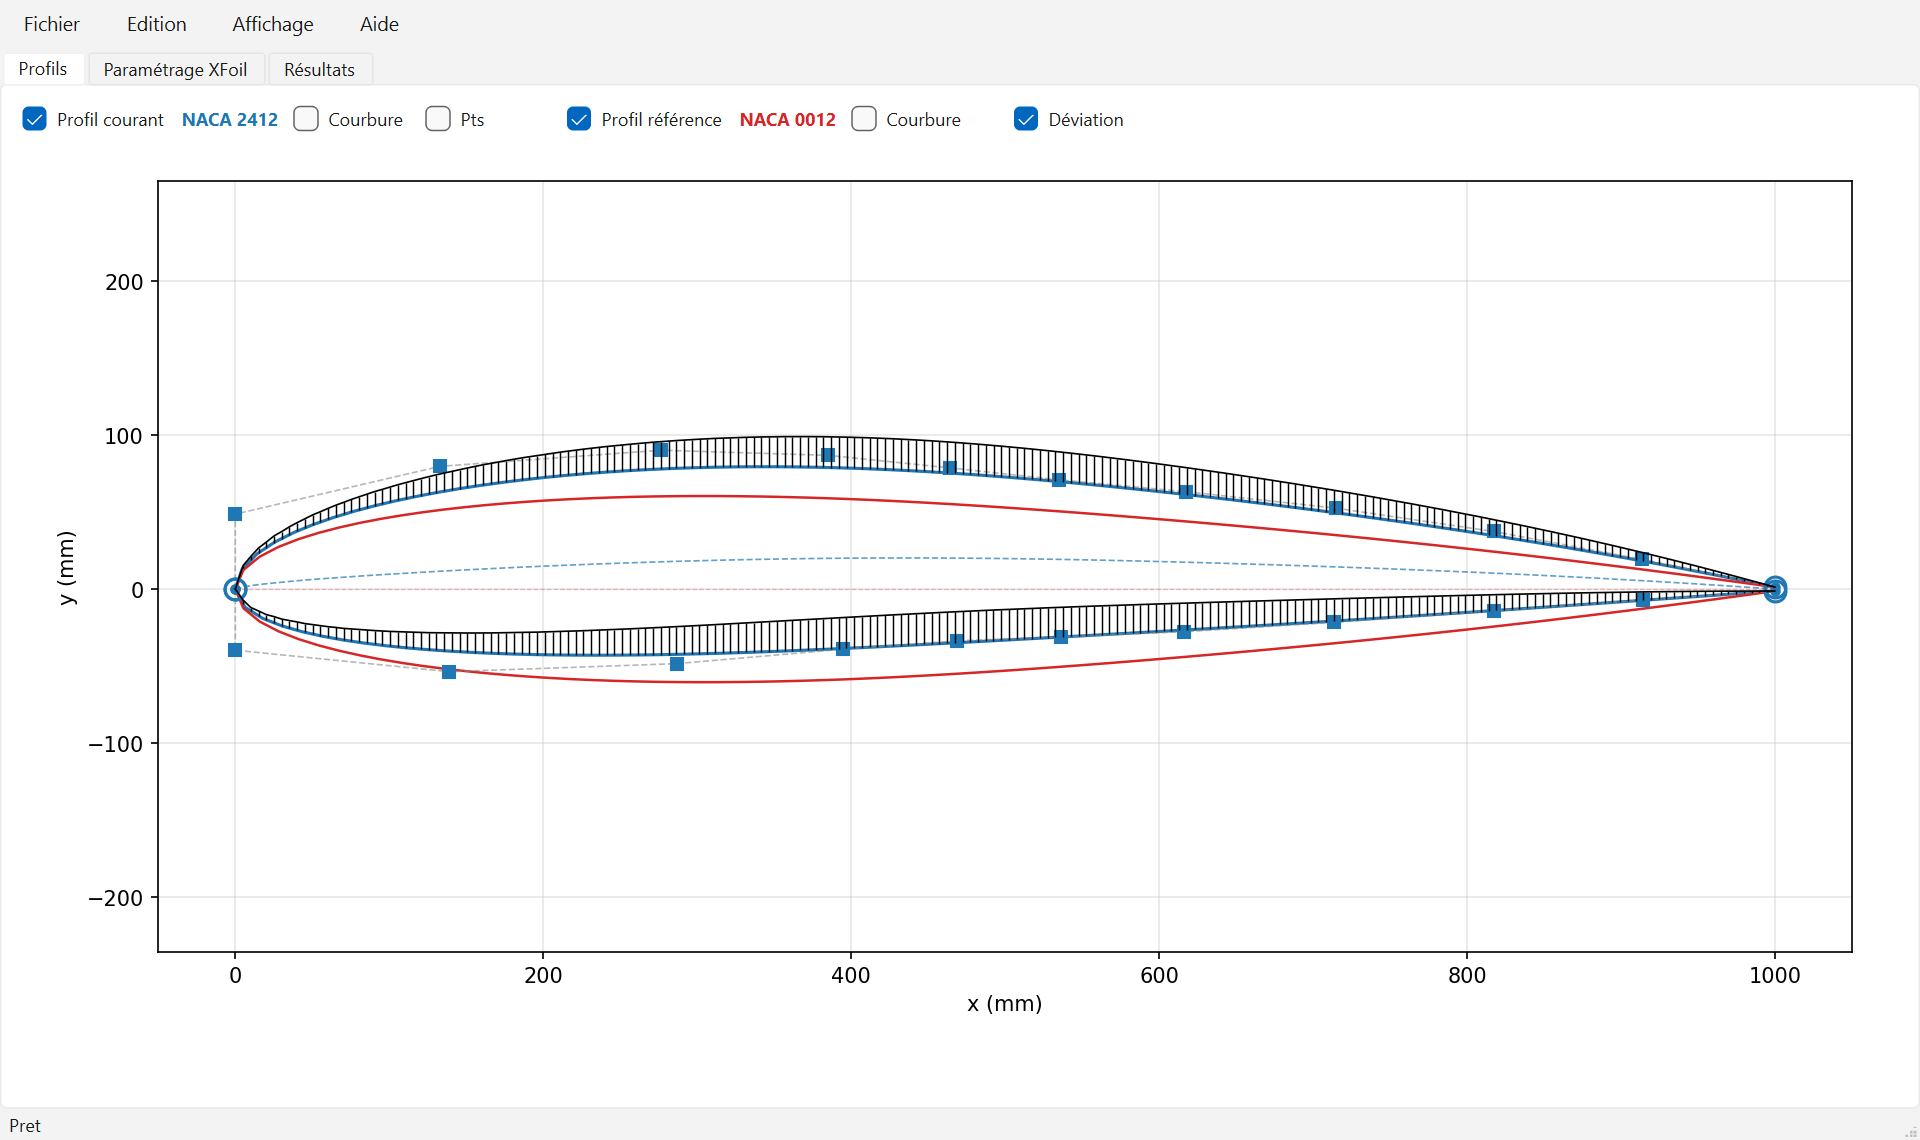
\includegraphics[width=0.49\textwidth]{images/06_tab_profils_deviation.png}}
    \hfill
    \fbox{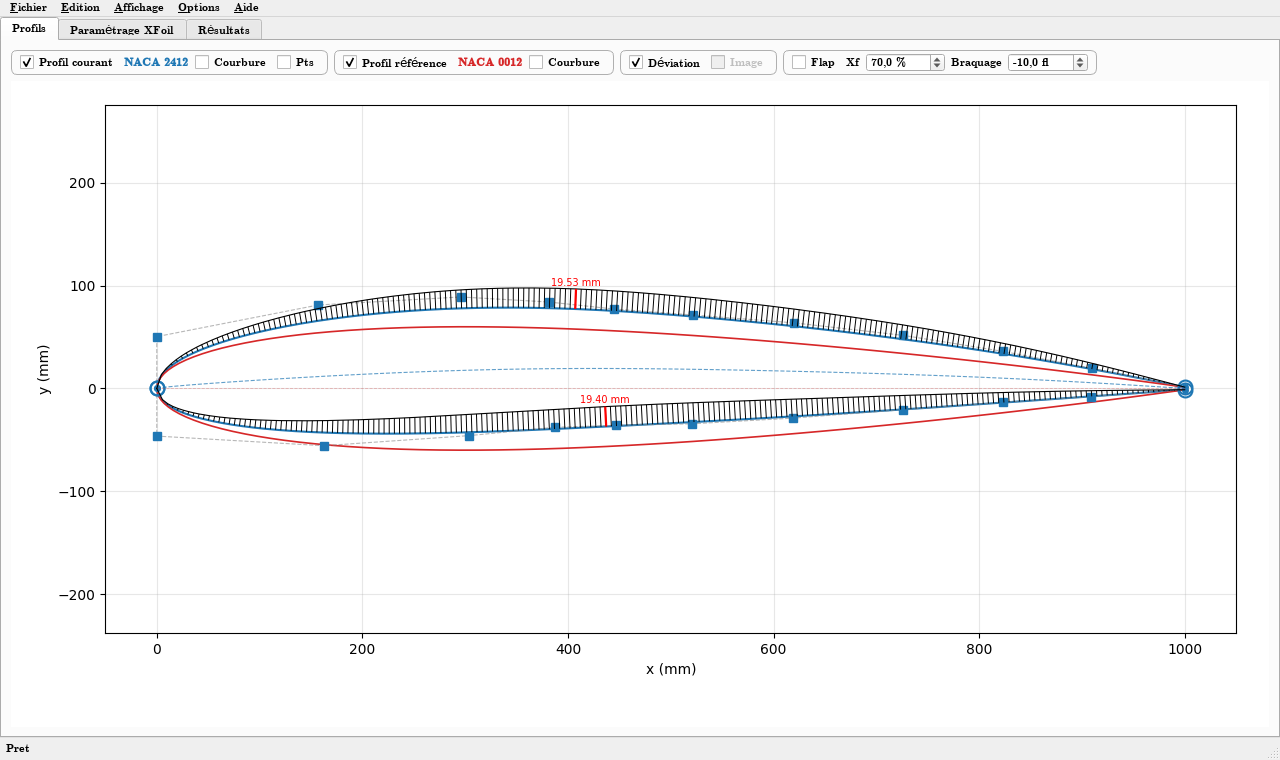
\includegraphics[width=0.49\textwidth]{images/14_deviation_normale.png}}
    \caption{Déviation entre NACA~2412 (courant, bleu) et NACA~0012
        (référence, rouge). À gauche le mode \emph{verticale}
        (quills verticaux), à droite le mode \emph{normale}
        (quills perpendiculaires à la surface). Dans les deux cas,
        le quill de déviation maximale est tracé en \textcolor{red}{rouge}
        avec sa valeur en millimètres.}
    \label{fig:06_tab_profils_deviation.png}
\end{figure}

\subsubsection*{Déviation maximale}

Le \textbf{maximum} de déviation est signalé par un quill
\textcolor{red}{\textbf{rouge}} portant sa \textbf{valeur en
millimètres} à son extrémité. Le calcul est effectué :

\begin{itemize}
    \item \textbf{par segment} de Bézier si le profil courant est en
        mode spline (un maximum par segment d'extrados et
        d'intrados) ;
    \item \textbf{par côté} (extrados, intrados) si le profil courant
        est en mode points discrets.
\end{itemize}

La valeur affichée est la déviation \textbf{réelle} (non
exagérée), exprimée dans l'unité du profil (millimètres pour une
corde de 1\,000~mm).

\begin{astuce}
Lorsque les profils ont une déviation très petite à l'œil
(par exemple lors d'une optimisation par petits déplacements
des points de contrôle), il est utile d'\textbf{amplifier}
l'affichage de la déviation. L'échelle est réglable via le
menu contextuel : \menu{Échelle déviation\dots}. Cette échelle
n'affecte que la longueur visuelle des quills, pas la valeur en
millimètres affichée au maximum.
\end{astuce}

\section{Charger un profil depuis la base UIUC}
\label{sec:uiuc}

AirfoilTools intègre un \textbf{accès direct} à la base de données
de profils de l'Université de l'Illinois (collection
\textbf{Selig}, environ 1\,600 profils), accessible via les entrées
\menu{Fichier $\rightarrow$ Depuis la base UIUC $\rightarrow$ Profil
courant\dots} et \menu{\dots Profil référence\dots}.

\screenshot{11_dialog_uiuc.png}{0.7}{%
    Dialogue de chargement depuis la base UIUC. La recherche
    \og naca \fg{} filtre 183~profils sur 1\,613. Le profil
    sélectionné affiche sa description sous la liste.}

\subsection{Utilisation}

\begin{enumerate}
    \item Au premier appel, l'index complet (~1\,600 profils) est
        téléchargé depuis le serveur UIUC. Le téléchargement prend
        quelques secondes selon la connexion.
    \item Saisir tout ou partie du nom ou de la description du
        profil dans le champ \menu{Recherche} : la liste se filtre
        en temps réel (insensible à la casse).
    \item Cliquer sur un profil pour voir sa description sous la
        liste. Double-clic ou bouton \bouton{Charger} pour le
        télécharger et l'ouvrir.
    \item Le profil est chargé en \textbf{mode points discrets}
        (format Selig). Pour bénéficier de l'édition interactive,
        utiliser ensuite \menu{Édition $\rightarrow$ Convertir en
        Spline} (voir section suivante).
\end{enumerate}

\subsection{Cache local}

Pour éviter de surcharger inutilement le serveur UIUC et pour
permettre l'utilisation hors ligne :

\begin{itemize}
    \item L'\textbf{index} (liste des profils + descriptions) est
        mis en cache pour \textbf{7~jours}. Au-delà, il est
        re-téléchargé automatiquement.
    \item Les \textbf{fichiers \chemin{.dat}} téléchargés sont mis
        en cache de manière \textbf{permanente} (les profils UIUC
        sont stables dans le temps).
\end{itemize}

Le bouton \bouton{Rafraichir} force le re-téléchargement de
l'index pour récupérer d'éventuels nouveaux profils.

L'emplacement du cache est :

\begin{itemize}
    \item Windows : \chemin{C:\textbackslash{}Users\textbackslash{}<utilisateur>\textbackslash{}.airfoiltools\textbackslash{}cache\textbackslash{}uiuc\textbackslash{}}
    \item Linux / macOS : \chemin{\textasciitilde/.airfoiltools/cache/uiuc/}
\end{itemize}

\begin{noteinfo}
Les fichiers \chemin{.dat} de la base UIUC suivent la
convention Selig (parcours BF $\rightarrow$ extrados $\rightarrow$
BA $\rightarrow$ intrados $\rightarrow$ BF) avec une ligne
d'en-tête contenant le nom du profil. Ils sont directement
exploitables par AirfoilTools.
\end{noteinfo}

\begin{attention}
Une connexion internet est requise pour le premier
téléchargement de l'index et de chaque profil. En cas
d'indisponibilité du serveur UIUC, le dialogue affiche un
message d'erreur ; les profils déjà mis en cache restent
toutefois utilisables.
\end{attention}

\section{Générer un profil NACA}
\label{sec:naca}

AirfoilTools sait générer à la volée les profils de la famille
\textbf{NACA} à partir de leur désignation, sans passer par un
fichier. La génération est accessible via \menu{Fichier
$\rightarrow$ Profil NACA $\rightarrow$ Profil courant\dots} (ou
\menu{\dots Profil référence\dots}).

\screenshot{16_dialog_naca.png}{0.55}{%
    Saisie des indices NACA. Un second dialogue demande ensuite le
    nombre de points du profil.}

\subsection{Utilisation}

\begin{enumerate}
    \item Saisir les \textbf{indices} dans le premier dialogue :
        \begin{itemize}
            \item \textbf{4 chiffres} (ex. \texttt{2412}) : cambrure
                maximale (\%), position de cambrure max (dixièmes de
                corde), épaisseur relative (\%) ;
            \item \textbf{5 chiffres} (ex. \texttt{23012}) : profil
                cambré à ligne moyenne plus complexe.
        \end{itemize}
    \item Saisir le \textbf{nombre de points} dans le second
        dialogue (par défaut 150).
    \item Le profil est généré, normalisé (corde 1\,000~mm) et
        affecté au rôle choisi (courant ou référence).
\end{enumerate}

\subsection{Régénération propre depuis le menu contextuel}

Un profil généré par cette fonction est \textbf{marqué} comme
profil NACA tant qu'il n'a pas été modifié (édition d'un point de
contrôle) ni converti en spline. Pour un tel profil NACA en mode
points discrets, le \textbf{menu contextuel} (clic droit) propose
l'entrée \menu{Nombre de points\dots}.

Changer le nombre de points par ce biais ne se contente pas
d'interpoler les points existants : il \textbf{rappelle la fonction
de génération NACA} pour produire un profil \emph{propre} à la
nouvelle résolution, conforme à la formule analytique.

\begin{noteinfo}
Cette régénération propre n'est possible que pour un profil NACA
\textbf{non modifié}. Dès qu'il est converti en spline ou édité,
le marqueur est perdu : on revient alors au ré-échantillonnage
classique de la spline.
\end{noteinfo}

\section{Conversion en spline}
\label{sec:convertspline}

Pour bénéficier de l'édition interactive, il faut convertir le
profil en mode spline. Cela se fait via :

\begin{itemize}
    \item le menu \menu{Édition $\rightarrow$ Convertir en Spline} ;
    \item le raccourci clavier \touche{Ctrl}+\touche{B}.
\end{itemize}

Un dialogue s'ouvre pour saisir les paramètres de conversion :

\screenshot{07_dialog_convert.png}{0.45}{%
    Dialogue de conversion en spline.}

\begin{tabularx}{\linewidth}{l X}
    \toprule
    \textbf{Paramètre} & \textbf{Description} \\
    \midrule
    Degré extrados
        & Degré des courbes de Bézier de l'extrados.
          Petit (3--5) = forme très lissée ; moyen (6--12) =
          compromis (recommandé) ; grand ($>$~15) = forme très
          précise mais risque d'oscillations.\\
    Degré intrados
        & Idem pour l'intrados. Peut être différent du degré
          extrados (typiquement intrados moins courbé).\\
    Tolérance
        & Déviation maximale acceptée entre la spline ajustée
          et les points discrets, en fraction de la corde.
          Valeur typique : $10^{-3}$ à $10^{-4}$.\\
    Max segments
        & Nombre maximal de segments de Bézier par côté.
          Avec 1, on obtient un seul segment global (comportement
          historique). Avec une valeur supérieure et une
          tolérance fine, l'algorithme \emph{adaptatif} découpe
          au point de plus grande erreur jusqu'à respecter la
          tolérance, concentrant les segments dans les zones de
          forte courbure (typiquement le bord d'attaque).\\
    Lissage
        & Coefficient de régularisation de l'ajustement
          (Tikhonov). $0$ = ajustement par moindres carrés pur ;
          $>0$ = lissage du polygone de contrôle.\\
    \bottomrule
\end{tabularx}

\begin{astuce}
Pour la plupart des profils, des paramètres de
\textbf{degré 11}, \textbf{tolérance $10^{-3}$},
\textbf{max segments 4}, \textbf{lissage 0{,}1} donnent un bon
compromis entre précision et qualité géométrique. Réduisez
la tolérance à $10^{-4}$ et augmentez \emph{Max segments} à
8--10 pour une approximation très fidèle.
\end{astuce}

\section{Édition interactive}

En mode spline, le canvas devient un \textbf{éditeur géométrique
interactif}.

\subsection{Interactions souris}

\begin{tabularx}{\linewidth}{l X}
    \toprule
    \textbf{Action} & \textbf{Effet} \\
    \midrule
    Clic gauche + déplacement sur un point de contrôle
        & Déplace le point de contrôle. La courbe est mise à
          jour en temps réel.\\
    Clic gauche + déplacement dans le vide
        & Trace un \emph{rectangle de zoom}. La vue est recadrée
          sur la zone à la fin du drag.\\
    Molette
        & Zoom centré sur la position du curseur.\\
    Clic milieu (ou \touche{Maj}+clic gauche)
        & Pan (translation de la vue).\\
    Clic droit
        & Ouvre le \textbf{menu contextuel}.\\
    \bottomrule
\end{tabularx}

\subsection{Menu contextuel (clic droit)}

Le menu contextuel offre plusieurs actions selon le contexte :

\begin{itemize}
    \item \menu{Info point\dots} (si clic sur un point de contrôle) :
        affiche les coordonnées et les paramètres locaux du point.
    \item \menu{Libérer la contrainte de tangence verticale au bord
        d'attaque} (si clic sur le nœud P1, voisin du bord d'attaque) :
        libère ou rétablit la tangente verticale au bord d'attaque.
        Voir la section~\ref{sec:batangente}.
    \item \menu{Échelle porcupines\dots} : règle l'échelle
        d'affichage de la courbure.
    \item \menu{Densité porcupines / $\times 2$ ou $\div 2$} :
        modifie le nombre de quills affichés.
    \item \menu{Échelle déviation\dots} et \menu{Densité déviation} :
        idem pour les porcupines de déviation.
    \item \menu{Split extrados / Split intrados} (en mode spline) :
        scinde la spline en deux au point cliqué le plus proche
        (algorithme de De Casteljau, exact).
    \item \menu{Paramètres globaux} : nombre de points
        d'échantillonnage, méthode (curviligne ou adaptative).
    \item \menu{Segment} (si clic dans un segment précis) :
        permet de définir des \emph{overrides per-segment}
        (degré, nombre de points, méthode différente du global).
\end{itemize}

\subsection{Tangente verticale au bord d'attaque}
\label{sec:batangente}

Par défaut, le premier point de contrôle intérieur de chaque côté
(noté \textbf{P1}, voisin du bord d'attaque) est \textbf{contraint}
à rester sur la verticale du bord d'attaque (BA). Cette contrainte
garantit une \textbf{tangente verticale} au bord d'attaque, ce qui
correspond à la géométrie naturelle de la plupart des profils. Lors
de l'édition, le déplacement de P1 est donc limité à l'axe vertical.

\screenshot{13_ba_tangente.png}{1.0}{%
    Effet de la contrainte de tangente verticale au bord d'attaque.
    À gauche, contrainte active : le nœud P1 (entouré en rouge) reste
    aligné verticalement avec le BA, la tangente (pointillé rouge) est
    verticale. À droite, contrainte libérée : P1 peut être déplacé
    librement, la tangente s'incline.}

Il est parfois souhaitable de \textbf{libérer} cette contrainte (par
exemple pour décalquer un profil dont le bord d'attaque n'a pas une
tangente strictement verticale). Pour cela :

\begin{enumerate}
    \item Effectuer un \textbf{clic droit} sur le nœud P1 de
        l'extrados ou de l'intrados.
    \item Choisir \menu{Libérer la contrainte de tangence verticale
        au bord d'attaque}.
\end{enumerate}

Le nœud P1 devient alors librement déplaçable (en $x$ et en $y$).
Pour rétablir la contrainte, refaire un clic droit sur le nœud et
choisir \menu{Rétablir la tangence verticale au bord d'attaque} :
le nœud P1 est automatiquement ramené sur la verticale du bord
d'attaque.

\begin{noteinfo}
La contrainte est gérée \textbf{indépendamment} pour l'extrados et
l'intrados. Libérer la tangente côté extrados n'affecte pas
l'intrados, et inversement.
\end{noteinfo}

\section{Volet (flap)}
\label{sec:flap}

Le module \textbf{volet} génère un \textbf{profil braqué} à partir
du profil courant, en faisant pivoter sa partie arrière autour d'un
axe d'articulation. Le profil avec volet est tracé en
\textbf{vert}, en plus du courant et de la référence ; il est
\textbf{non modifiable} (recalculé automatiquement) et peut être
simulé puis sauvegardé comme le profil courant.

\screenshot{15_tab_profils_flap.png}{1.0}{%
    Profil avec volet (vert) braqué à $-10^\circ$ à 70~\% de corde,
    superposé au profil courant (bleu) et à ses points de contrôle.}

\subsection{Activation et réglages}

Les contrôles se trouvent dans le cadre \og Flap \fg{} de la barre
de l'onglet \menu{Profils} :

\begin{tabularx}{\linewidth}{l X}
    \toprule
    \textbf{Contrôle} & \textbf{Rôle} \\
    \midrule
    \textbf{Flap} & Active la génération du profil braqué (vert). \\
    \textbf{Xf} & Position de l'axe d'articulation, en \textbf{pourcent
        de corde} mesuré depuis le bord d'attaque (5 à 95~\%). \\
    \textbf{Braquage} & Angle de braquage en degrés ($-45$ à
        $+45$). \textbf{Positif} = bord de fuite vers le \textbf{haut} ;
        \textbf{négatif} = bord de fuite vers le \textbf{bas}. \\
    \bottomrule
\end{tabularx}

Le profil braqué est recalculé en temps réel à chaque changement
de \menu{Xf} ou de \menu{Braquage}, et à chaque modification du
profil courant.

\subsection{Géométrie de l'articulation}

L'axe d'articulation est le \textbf{centre du cercle inscrit}
tangent simultanément à l'extrados et à l'intrados, dont l'abscisse
vaut \menu{Xf}. La partie arrière de chaque surface est ensuite
tournée de l'angle de braquage autour de cet axe.

\screenshot{19_flap_schema.png}{0.95}{%
    Construction de l'articulation : le cercle inscrit (vert),
    tangent à l'extrados et à l'intrados à l'abscisse $X_f$, fournit
    le centre de rotation (point rouge) du volet.}

Selon le côté et le signe du braquage, le raccord entre la partie
fixe et la partie braquée est traité différemment :

\begin{itemize}
    \item du côté où le braquage \textbf{ouvre} un jeu, un
        \textbf{arc de cercle} comble l'espace ;
    \item du côté où le braquage \textbf{referme} la matière, la
        surface est \textbf{coupée à l'intersection} (recouvrement
        retiré).
\end{itemize}

\subsection{Simulation et sauvegarde}

\begin{itemize}
    \item \textbf{Simulation} : le profil avec volet est simulé par
        XFoil au même titre que le courant et la référence. Le bouton
        \bouton{Flap seul} de l'onglet \menu{Paramétrage XFoil} le
        calcule isolément ; \bouton{Lancer tout} l'inclut s'il est
        actif. Les résultats apparaissent sous le rôle
        \emph{Volet} (vert) dans l'onglet \menu{Résultats}.
    \item \textbf{Sauvegarde} : \menu{Fichier $\rightarrow$
        Sauvegarder profil avec volet\dots} enregistre le profil
        braqué, avec le même choix complet / extrados / intrados et
        les mêmes formats que le profil courant.
\end{itemize}

\begin{important}
Pour la simulation, le profil avec volet est exprimé dans le
\textbf{repère normalisé du profil courant} : XFoil ne le
renormalise ni ne le redresse. On observe ainsi uniquement
l'effet du braquage par rapport au profil courant (déplacement de
la polaire, du moment, etc.), sans artefact de changement de corde
ou d'incidence de référence.
\end{important}

\section{Image de calque (décalquer un profil)}
\label{sec:calque}

AirfoilTools permet de charger une \textbf{image en arrière-plan}
(photo, scan d'un plan, capture d'écran d'un profil) afin de
\textbf{décalquer} sa forme en déplaçant les points de contrôle du
profil courant jusqu'à épouser la silhouette de l'image.

\screenshot{12_tab_profils_calque.png}{1.0}{%
    Décalquage d'un profil : l'image de calque (silhouette grise) est
    affichée en arrière-plan ; le profil courant (bleu, en mode spline)
    et ses points de contrôle se superposent par-dessus. On ajuste les
    points de contrôle pour faire coïncider la courbe bleue avec la
    silhouette.}

\subsection{Chargement de l'image}

Le chargement se fait via \menu{Fichier $\rightarrow$ Charger image
de calque\dots}. Les formats usuels sont acceptés : \chemin{.jpg},
\chemin{.png}, \chemin{.tif}, \chemin{.bmp}. À l'ouverture, l'image
est mise à l'échelle pour couvrir approximativement la corde
(1\,000~mm) et la case \textbf{Image} de la barre de contrôle
devient active et cochée.

L'image est dessinée \textbf{en arrière-plan}, sous le profil et ses
points de contrôle, qui restent donc parfaitement visibles et
manipulables par-dessus.

\subsection{Positionner, mettre à l'échelle et tourner l'image}

Les manipulations de l'image se font en maintenant la touche
\touche{i} enfoncée, combinée à la souris :

\begin{tabularx}{\linewidth}{l X}
    \toprule
    \textbf{Action} & \textbf{Effet} \\
    \midrule
    \touche{i} + clic gauche glissé
        & \textbf{Déplace} l'image (translation).\\
    \touche{i} + molette
        & \textbf{Met à l'échelle} l'image (agrandit / réduit autour
          de son centre).\\
    \touche{i} + clic droit glissé
        & \textbf{Tourne} l'image autour de l'origine $(0,0)$
          (le bord d'attaque).\\
    \touche{Maj} + \touche{i} + action
        & \textbf{Ajustements fins} : déplacement et rotation
          dix fois plus lents, pas d'échelle réduit. Idéal pour le
          calage précis.\\
    \bottomrule
\end{tabularx}

\begin{astuce}
Procédez en deux temps : d'abord un calage grossier (déplacement,
échelle, rotation sans \touche{Maj}) pour superposer
approximativement l'image et le profil, puis un \textbf{ajustement
fin} en maintenant \touche{Maj} pour le calage précis du bord
d'attaque et du bord de fuite.
\end{astuce}

\begin{noteinfo}
Le canvas doit avoir le \textbf{focus clavier} pour que la touche
\touche{i} soit prise en compte : il l'obtient automatiquement
dès que le curseur survole la zone de tracé.
\end{noteinfo}

\subsection{Masquer ou retirer l'image}

\begin{itemize}
    \item La case \textbf{Image} de la barre de contrôle affiche ou
        masque l'image sans la supprimer.
    \item \menu{Fichier $\rightarrow$ Retirer l'image de calque}
        supprime définitivement l'image de la session.
\end{itemize}

\begin{important}
L'image de calque et sa position (échelle, rotation, translation)
sont \textbf{enregistrées avec le projet} au format \chemin{.aftproj}
(voir chapitre~\ref{chap:formats}). On retrouve ainsi son calque
exactement tel qu'il était à la réouverture du projet. Les formats
de profil classiques (\chemin{.dat}, \chemin{.bspl}\dots) ne
contiennent \textbf{pas} l'image : pour conserver le calque, il faut
enregistrer un projet.
\end{important}

\section{Avertissement \og Courbure indisponible \fg{}}

Lorsque la case \menu{Courbure} est activée alors que le profil
concerné est en mode points discrets (non converti en spline),
un message d'information s'affiche :

\screenshot{08_msg_courbure.png}{0.7}{%
    Message d'avertissement \og Courbure indisponible \fg{}.}

Comme indiqué dans le message, deux solutions sont possibles :

\begin{enumerate}
    \item convertir le profil en spline (menu
        \menu{Édition $\rightarrow$ Convertir en Spline}) ;
    \item charger un profil dans un format préservant la
        géométrie spline (\chemin{.bspl} ou \chemin{.bez}).
\end{enumerate}

La case se décoche automatiquement après affichage du message.

\section{Modification du nombre de points}

En mode spline, le nombre de points d'échantillonnage discret
des splines est modifiable via le menu \menu{Édition $\rightarrow$
Échantillonnage $\rightarrow$ Profil courant\dots} (ou
\menu{\dots Profil référence\dots}).

Un dialogue demande le nouveau nombre de points (entre 10 et
10\,000). Cela affecte uniquement la \emph{discrétisation
d'export} et l'affichage : la géométrie spline sous-jacente
n'est pas altérée.

\begin{noteinfo}
Pour les simulations XFoil, l'échantillonnage par défaut
(150~points) est généralement suffisant. XFoil ré-échantillonne
ensuite en interne via la commande \texttt{PANE} si l'option
\emph{Repanel} est activée dans l'onglet \menu{Paramétrage XFoil}.
\end{noteinfo}

\chapter{Onglet Paramétrage XFoil}
\label{chap:xfoil}

L'onglet \menu{Paramétrage XFoil} regroupe l'ensemble des paramètres
de simulation transmis au solveur. Il est structuré en zones de
saisie (Reynolds, Alpha, Paramètres XFoil), une rangée de boutons
de lancement et un cadre \menu{Diagnostic}.

\screenshot{09_tab_xfoil.png}{1.0}{%
    Onglet \menu{Paramétrage XFoil} : zones de saisie, boutons de
    lancement (dont \og Flap seul \fg{}) et cadre \og Diagnostic \fg{}.}

\begin{noteinfo}
Valeurs par défaut au démarrage : Reynolds de 1\,000\,000 à
2\,000\,000 (pas 1\,000\,000), incidence de $-5^\circ$ à $+15^\circ$
(pas $0{,}5^\circ$), transition forcée XTR~$=0{,}2$, 100~itérations,
balayage \menu{ASEQ}.
\end{noteinfo}

\begin{noteinfo}
Ces paramètres alimentent le \textbf{solveur sélectionné} dans
\menu{Options $\rightarrow$ Solveur} (XFoil ou FlexFoil, voir
chapitre~\ref{chap:interface}). Les deux moteurs interprètent les mêmes
réglages ; certaines options propres à l'exécutable XFoil (balayage
\menu{ASEQ}, réinitialisation en cas d'échec) n'ont pas d'effet sur
FlexFoil, qui converge par une méthode native.
\end{noteinfo}

\section{Plage de Reynolds}

La zone \menu{Reynolds} permet de définir une \textbf{plage} de
nombres de Reynolds pour le balayage. Pour chaque Reynolds, une
polaire complète est calculée. Trois champs :

\begin{tabularx}{\linewidth}{l X}
    \toprule
    \textbf{Champ} & \textbf{Description} \\
    \midrule
    Min  & Reynolds minimum du balayage. \\
    Max  & Reynolds maximum du balayage. \\
    Pas  & Incrément entre deux valeurs consécutives. Pour
           ne calculer qu'un seul Reynolds, choisir
           \texttt{Pas $\geq$ Max - Min}. \\
    \bottomrule
\end{tabularx}



\section{Plage d'incidence (Alpha)}

La zone \menu{Alpha (deg)} définit le balayage en angle d'incidence
$\alpha$ pour chaque polaire :

\begin{tabularx}{\linewidth}{l X}
    \toprule
    \textbf{Champ} & \textbf{Description} \\
    \midrule
    Min  & Incidence minimum (en degrés, peut être négative). \\
    Max  & Incidence maximum. \\
    Pas  & Incrément entre deux points de la polaire. Plus
           petit~=~polaire plus fine, mais simulation plus longue.\\
    \bottomrule
\end{tabularx}

\subsection*{Mode \menu{ASEQ}}

La case à cocher \menu{ASEQ} contrôle la \textbf{stratégie de
balayage} en incidence~:

\begin{itemize}
    \item \textbf{Cochée} (par défaut) : XFoil exécute la commande
        \texttt{ASEQ} qui balaye automatiquement la plage en
        partant du minimum. C'est le mode \emph{rapide} historique.
    \item \textbf{Décochée} : AirfoilTools envoie une succession de
        commandes \texttt{ALFA} individuelles, en partant de
        $\alpha=0$ vers le maximum, puis depuis $-\Delta$ vers le
        minimum (avec une commande \texttt{INIT} entre les deux).
        Ce mode est plus \emph{robuste} à la convergence aux
        angles élevés ou pour des profils difficiles.
\end{itemize}

\begin{astuce}
Si XFoil ne converge pas pour certains angles élevés, désactivez
\menu{ASEQ} pour tenter le balayage bidirectionnel. Cela
améliore souvent la convergence en initialisant chaque branche
à partir de la solution à $\alpha=0$.
\end{astuce}

\subsection*{Option \menu{Réinit. si échec}}

Lorsqu'un point d'incidence ne converge pas (message
\texttt{VISCAL: Convergence failed}), le balayage en marche peut
\textbf{abandonner toute la suite} de la branche (effet de cascade).
La case \menu{Réinit. si échec} ajoute une \textbf{seconde passe}
qui rejoue chaque incidence depuis un état propre (commande
\texttt{INIT} avant chaque \texttt{ALFA}), afin de récupérer les
points manqués sans dégrader le balayage en marche (le
postprocesseur conserve la solution obtenue en marche lorsqu'elle
existe).

\begin{attention}
L'option \menu{Réinit. si échec} implique le mode \texttt{ALFA}
individuel (incompatible avec \menu{ASEQ}) et \textbf{double
environ} le temps de calcul. Pensez à augmenter le \menu{Timeout}
en conséquence. Elle est \textbf{décochée par défaut}.
\end{attention}

\section{Paramètres XFoil avancés}

La zone \menu{Paramètres XFoil} regroupe les options du solveur
proprement dit.

\subsection{Viscosité}

\begin{itemize}
    \item Cochée (\menu{Avec}) : analyse \textbf{visqueuse}
        (commande \texttt{VISC} de XFoil), avec couche limite.
        \textbf{Recommandé pour toute polaire réaliste.}
    \item Décochée : analyse non-visqueuse (potentielle, sans
        frottement). Utile uniquement pour des comparaisons
        géométriques rapides.
\end{itemize}

\subsection{NCRIT}

Critère de transition de couche limite par la méthode $e^N$
(amplification des ondes de Tollmien-Schlichting).

\begin{tabularx}{\linewidth}{c X}
    \toprule
    \textbf{NCRIT} & \textbf{Type d'écoulement} \\
    \midrule
    9       & Écoulement libre standard (valeur par défaut). \\
    4--7    & Écoulement très turbulent (souffleries fermées,
              forte turbulence ambiante). \\
    12--14  & Écoulement très calme (vol planeur en air
              parfaitement laminaire). \\
    \bottomrule
\end{tabularx}

\subsection{XTR Top et XTR Bot}

Position de \textbf{transition forcée} de la couche limite,
respectivement sur l'extrados (\emph{top}) et l'intrados
(\emph{bottom}), exprimée en fraction de corde ($x/c$).

\begin{itemize}
    \item Valeur 1{,}0 : transition libre, calculée par le critère
        NCRIT. C'est le mode standard.
    \item Valeur $<1{,}0$ : transition forcée à la position indiquée
        (simule un \emph{trip} turbulent : turbulateur, rugosité,
        impact d'insectes\dots).
\end{itemize}

\begin{important}
La valeur minimale est \textbf{0{,}05}. Forcer la transition trop
près du bord d'attaque (par exemple 0{,}01) \textbf{déstabilise la
couche limite de XFoil} : la routine de transition diverge
(\texttt{NaN}) et entre dans une boucle quasi infinie, jusqu'à
expiration du \menu{Timeout}. La valeur par défaut est
\textbf{0{,}2}.
\end{important}

\subsection{Repanel et NPanel}

\begin{itemize}
    \item \menu{Repanel} : si cochée, XFoil exécute la commande
        \texttt{PANE} qui ré-échantillonne le profil avec un
        critère adaptatif basé sur la courbure. Recommandé pour
        les profils à échantillonnage non-uniforme ou pour des
        profils de très haute résolution.
    \item \menu{NPanel} : nombre de panneaux après ré-échantillonnage
        (par défaut 200). Plus = plus précis mais plus lent.
\end{itemize}

\subsection{Timeout}

Durée maximale d'exécution de XFoil pour le calcul d'une polaire,
en secondes (par défaut 30~s). Au-delà, le processus est tué.
Cela évite à l'application de rester bloquée si XFoil entre dans
une boucle de non-convergence.

\begin{attention}
Augmenter le timeout (par exemple à 120~s) si vous balayez une
plage très large d'incidences ($\Delta \alpha > 30^\circ$), si vous
calculez plusieurs Reynolds, si l'option \menu{Réinit. si échec}
est active (temps doublé), ou si vos profils convergent lentement.
\end{attention}

\subsection{Itérations}

Nombre maximum d'itérations de Newton par point (commande
\texttt{ITER} de XFoil), par défaut 100. \textbf{Augmenter} cette
valeur (200--300) lorsqu'un point précis ne converge pas
(\texttt{VISCAL: Convergence failed}), situation typique près du
décrochage ou avec un coude de volet.

\section{Boutons de lancement}

Quatre boutons en bas de la zone de paramètres permettent de lancer
la simulation :

\begin{itemize}
    \item \bouton{Lancer tout} : simule tous les profils actifs ---
        courant, référence et, si le volet est activé, le profil
        avec volet.
    \item \bouton{Courant seul} : ne simule que le profil courant
        (bleu).
    \item \bouton{Référence seul} : ne simule que le profil de
        référence (rouge).
    \item \bouton{Flap seul} : ne simule que le profil avec volet
        (vert). Nécessite que le volet soit activé dans l'onglet
        \menu{Profils}.
\end{itemize}

Pendant la simulation, les contrôles de l'onglet sont désactivés,
et une \textbf{barre de progression} apparaît dans la barre de
statut : déterminée (un cran par profil terminé) lorsque plusieurs
profils sont simulés, sinon indéterminée (animation « busy »), car un
balayage en incidence s'exécute en un seul calcul sans avancement
intermédiaire. À la fin, l'onglet \menu{Résultats} se sélectionne
automatiquement.

\begin{important}
Si vous relancez une simulation pour \textbf{un seul} des profils,
les résultats antérieurs des autres profils sont \emph{conservés}
(merge). Cela permet par exemple d'itérer rapidement sur le profil
courant tout en gardant la référence fixe pour comparaison.
\end{important}

\section{Diagnostic}
\label{sec:diagnostic}

Le cadre \menu{Diagnostic}, en bas de l'onglet, donne accès aux
fichiers internes de la dernière simulation de chaque profil
(\bouton{Courant}, \bouton{Référence}, \bouton{Volet}). Les
boutons restent inactifs tant qu'aucune simulation n'a été lancée
pour le profil correspondant.

\screenshot{17_dialog_diagnostic.png}{0.85}{%
    Fenêtre de diagnostic : accès au répertoire de travail et aux
    fichiers de la simulation. Le journal \chemin{diagnostic.log}
    récapitule le déroulé du calcul.}

La fenêtre de diagnostic permet de :

\begin{itemize}
    \item parcourir les \textbf{fichiers} de la simulation : journal
        \chemin{diagnostic.log} (résumé du déroulé : étapes,
        avertissements, bilan de convergence), log console XFoil
        (\chemin{xfoil\_alpha.cmd.log}), script de commandes,
        polaires, distributions de pression ;
    \item \textbf{ouvrir le dossier} de travail dans l'explorateur
        de fichiers du système.
\end{itemize}

\begin{astuce}
En cas d'échec ou de résultats incomplets, ouvrez d'abord
\chemin{diagnostic.log} : il indique clairement si le problème
vient d'une non-convergence (\og AUCUN point convergé\dots\fg{}),
d'un \emph{timeout}, ou d'une polaire vide. Le log console XFoil
fournit ensuite le détail incidence par incidence. Le journal est
sauvegardé \textbf{même en cas de timeout}.
\end{astuce}

\chapter{Onglet Résultats}
\label{chap:resultats}

L'onglet \menu{Résultats} présente les résultats de simulation
sous forme d'une \textbf{grille configurable de cellules
d'analyse}. Chaque cellule affiche un type de tracé indépendant
(polaire, distribution de pression, profil de couche limite,
etc.).

\screenshot{10_tab_results_empty.png}{1.0}{%
    Onglet \menu{Résultats} avant toute simulation. La grille
    est par défaut en disposition $2\times2$, soit
    quatre cellules vides.}

\screenshot{18_tab_results.png}{1.0}{%
    Onglet \menu{Résultats} après simulation du profil courant
    (bleu), de la référence (rouge) et du profil avec volet (vert).
    Les quatre cellules affichent ici $C_L(\alpha)$, la polaire
    $C_L(C_D)$, la finesse $C_L/C_D$ en fonction de $C_L$ et le
    moment $C_M(C_L)$.}

\section{Configuration de la grille}

La grille est configurable via le menu
\menu{Affichage $\rightarrow$ Disposition}. Cinq dispositions
préconfigurées sont disponibles : $1\times1$, $1\times2$,
$2\times2$ (par défaut), $2\times3$, $3\times3$.

\begin{noteinfo}
Lors d'un changement de disposition, les analyses déjà
sélectionnées dans les cellules existantes sont conservées.
Les nouvelles cellules sont initialisées avec les analyses
par défaut.
\end{noteinfo}

\section{Cellule d'analyse}

Chaque cellule comporte une \textbf{barre de contrôle} et un
\textbf{canvas matplotlib}.

\subsection{Barre de contrôle}

\begin{tabularx}{\linewidth}{l X}
    \toprule
    \textbf{Élément} & \textbf{Rôle} \\
    \midrule
    Liste déroulante (analyse)
        & Choix du type d'analyse à afficher dans la cellule
          (voir \emph{Types d'analyse}, ci-après). \\
    Case \menu{C}
        & Affiche / masque les courbes du profil courant (bleu). \\
    Case \menu{R}
        & Affiche / masque les courbes du profil de référence (rouge). \\
    Case \menu{F}
        & Affiche / masque les courbes du profil avec volet (vert). \\
    Liste \menu{Reynolds}
        & Pour les analyses dépendant d'un Reynolds particulier
          ($-C_p(x)$, Cp~+~Profil, profil~+~CL), choisit le
          Reynolds à afficher. Masquée si non pertinente. \\
    Liste \menu{Alpha}
        & Pour les analyses dépendant d'une incidence (Cp~+~Profil,
          profil~+~CL et les grandeurs de couche limite), choisit
          l'incidence $\alpha$ à afficher. Masquée si non pertinente. \\
    Coordonnées
        & Affichage en temps réel des coordonnées du curseur
          dans le repère du graphique. \\
    \bottomrule
\end{tabularx}

\subsection{Interactions souris}

Les interactions disponibles sur le canvas matplotlib sont
identiques à celles de l'onglet \menu{Profils} :

\begin{itemize}
    \item Clic gauche + drag : zoom rectangle ;
    \item Molette : zoom centré sur le curseur ;
    \item Clic milieu : pan ;
    \item Clic gauche sur la légende : masque / réaffiche la
        courbe correspondante.
\end{itemize}

\subsection{Légende interactive et défilante}

Lorsqu'une cellule contient de nombreuses courbes (par exemple
plusieurs Reynolds combinés à plusieurs profils), la légende peut
devenir trop longue pour s'afficher entièrement. Une \textbf{barre
de défilement} apparaît automatiquement au-delà de 15~entrées.

\begin{astuce}
Pour comparer rapidement deux courbes, il est plus efficace
de \textbf{masquer} les courbes parasites en cliquant sur leur
entrée dans la légende, plutôt que de zoomer ou d'ajouter
une cellule supplémentaire.
\end{astuce}

\section{Types d'analyse disponibles}

\subsection{Polaires (en fonction d'Alpha)}

\begin{tabularx}{\linewidth}{l X}
    \toprule
    \textbf{Analyse} & \textbf{Description} \\
    \midrule
    $C_L(\alpha)$  & Coefficient de portance en fonction de
                     l'incidence. Une courbe par Reynolds.\\
    $C_D(\alpha)$  & Coefficient de traînée en fonction de
                     l'incidence.\\
    $C_M(\alpha)$  & Coefficient de moment de tangage
                     (référence quart de corde).\\
    $C_L/C_D$~$(\alpha)$ & \emph{Finesse} en fonction de
                     l'incidence. Permet de déterminer
                     l'incidence de finesse maximale.\\
    $C_L/C_D$~$(C_L)$ & \emph{Finesse} en fonction du coefficient de
                     portance. Pratique pour lire la finesse au
                     $C_L$ de croisière visé.\\
    $C_M(C_L)$     & Coefficient de moment en fonction de la
                     portance. La pente renseigne sur la stabilité ;
                     l'effet d'un volet y est très lisible.\\
    $C_D(C_L)$ \emph{(polaire de Lilienthal)}
                   & Polaire classique : traînée en abscisse
                     vs portance en ordonnée. La tangente
                     depuis l'origine donne la finesse maximale.\\
    Transition top, bot
                   & Position $x/c$ de la transition de couche
                     limite sur extrados / intrados, en fonction
                     de $\alpha$. Renseigne sur la rugosité
                     effective et le décrochage laminaire.\\
    \bottomrule
\end{tabularx}

\subsection{Distributions le long du profil}

\begin{tabularx}{\linewidth}{l X}
    \toprule
    \textbf{Analyse} & \textbf{Description} \\
    \midrule
    $-C_p(x)$ & Distribution du coefficient de pression le long
               de la corde, à un Reynolds et une incidence donnés.
               Convention : $-C_p$ vers le haut (extrados au-dessus). \\
    Cp + Profil & Tracé combiné façon \emph{XFoil} : le $-C_p$ en haut
               et le profil redessiné en dessous, pour un couple
               (Reynolds, incidence). Un encart résume les coefficients
               ($C_L$, $C_M$, $C_D$, finesse). Pour une vue dédiée plus
               complète (Cp non visqueux et couche limite), voir le
               chapitre~\ref{chap:cp}. \\
    Profil + CL & Visualisation combinée : profil tourné par
               l'incidence + tracé de la frontière de couche
               limite (épaisseur de déplacement $\delta^*$).\\
    \bottomrule
\end{tabularx}

\subsection{Couche limite}

Cinq grandeurs de couche limite peuvent être tracées en fonction
de l'abscisse curviligne $s$ ou de l'abscisse cartésienne $x$. Elles
sont évaluées à l'\textbf{incidence sélectionnée} (liste \menu{Alpha})
— la couche limite étant calculée pour chaque $\alpha$ — et chaque
courbe compare les Reynolds disponibles :

\begin{tabularx}{\linewidth}{l X}
    \toprule
    \textbf{Grandeur} & \textbf{Description} \\
    \midrule
    $U_e(s)$, $U_e(x)$
        & Vitesse au bord de la couche limite,
          normalisée par la vitesse infinie amont.\\
    $\delta^*(s)$, $\delta^*(x)$
        & Épaisseur de déplacement.\\
    $\theta(s)$, $\theta(x)$
        & Épaisseur de quantité de mouvement.\\
    $C_f(s)$, $C_f(x)$
        & Coefficient de frottement local.\\
    $H(s)$, $H(x)$
        & Facteur de forme $H = \delta^*/\theta$ ($H \approx 2{,}6$
          au point de transition, $H \approx 4$ au décollement).\\
    \bottomrule
\end{tabularx}

\section{Bandeau de résultats obsolètes}

Lorsque l'utilisateur revient à l'onglet \menu{Profils} et modifie
un profil après simulation (déplacement d'un point de contrôle,
changement de degré, conversion\dots), un bandeau jaune apparaît
en haut de l'onglet \menu{Résultats} :

\begin{quote}
\textcolor{orange!75!black}{$\triangle$
\emph{Le profil courant a été modifié depuis la dernière
simulation. Relancez pour mettre à jour.}}
\end{quote}

Ce bandeau disparaît automatiquement à la prochaine simulation.

\begin{important}
Les résultats affichés dans les cellules \emph{ne sont pas}
recalculés automatiquement après modification d'un profil.
Le bandeau est un simple indicateur visuel : il appartient
à l'utilisateur de relancer la simulation depuis l'onglet
\menu{Paramétrage XFoil}.
\end{important}

\chapter{Formats de fichiers}
\label{chap:formats}

AirfoilTools sait lire et écrire plusieurs formats de profil, qui
se répartissent en deux familles : les formats \emph{points
discrets} (issus du milieu aéronautique) et les formats
\emph{splines} propres à AirfoilTools.

\section{Formats points discrets}

\subsection{Format Selig (\chemin{.dat})}

Format historique le plus répandu, popularisé par la base de
données de l'Université de l'Illinois (UIUC). C'est le format
par défaut sur \chemin{airfoiltools.com}.

\begin{itemize}
    \item Première ligne : nom du profil (libre).
    \item Lignes suivantes : couples \texttt{x y} séparés par
        des espaces.
    \item Parcours en \emph{convention Selig} : du bord de fuite
        ($x=1$) vers l'extrados (x décroissant), au bord
        d'attaque ($x=0$), puis vers l'intrados (x croissant)
        et retour au bord de fuite.
\end{itemize}

\begin{lstlisting}[caption={Exemple de fichier Selig (NACA~2412)}]
NACA 2412
   1.000000   0.001260
   0.985700   0.003930
   0.971440   0.006580
   ...
   0.014300   0.018780
   0.000000   0.000000
   0.014300  -0.014050
   ...
   0.985700  -0.001280
   1.000000  -0.001260
\end{lstlisting}

\subsection{Format Lednicer (\chemin{.dat})}

Variante du Selig où extrados et intrados sont stockés
séparément, chacun parcouru du bord d'attaque vers le bord de
fuite. Une ligne d'en-tête indique le nombre de points de chaque
côté.

\begin{lstlisting}[caption={Exemple de fichier Lednicer}]
NACA 2412
65.0   65.0

   0.000000   0.000000
   0.001425   0.005700
   ...
   1.000000   0.001260

   0.000000   0.000000
   0.001425  -0.005720
   ...
   1.000000  -0.001260
\end{lstlisting}

\subsection{Format CSV (\chemin{.csv})}

Format tabulaire avec en-tête \chemin{x,y}. Pratique pour
l'import dans des feuilles de calcul ou pour le partage avec des
outils non-aéronautiques.

\begin{lstlisting}[caption={Exemple de fichier CSV}]
x,y
1.000000,0.001260
0.985700,0.003930
...
\end{lstlisting}

\section{Formats splines AirfoilTools}

\subsection{Format \chemin{.bspl}}

Sauvegarde complète d'un profil en mode \textbf{spline
multi-segment}. Préserve l'intégralité de la définition Bézier :
points de contrôle, degrés, continuités aux jonctions, paramètres
d'échantillonnage.

C'est le format \textbf{recommandé} pour conserver le travail
d'édition d'un profil et le ré-ouvrir sans perte d'information.

\begin{noteinfo}
Le format \chemin{.bspl} est un format texte structuré (JSON
ou similaire) propre à AirfoilTools. Il n'est pas
interopérable avec d'autres logiciels de CAO ou
d'aérodynamique. Pour une diffusion externe, ré-exportez en
\chemin{.dat} (Selig) après avoir ajusté l'échantillonnage.
\end{noteinfo}

\subsection{Format \chemin{.bez}}

Variante simplifiée du \chemin{.bspl} pour les profils définis
par une seule courbe de Bézier par côté (mode mono-segment).
Conservé pour compatibilité avec les versions antérieures.

\section{Génération NACA}

L'application sait générer à la volée des profils NACA à partir
de leur désignation, sans passer par un fichier :

\begin{itemize}
    \item NACA 4 chiffres (ex. \texttt{2412}, \texttt{0012}) :
        cambrure maximale (\%), position de la cambrure max
        (dixièmes), épaisseur relative (\%).
    \item NACA 5 chiffres (ex. \texttt{23012}) : profil cambré
        avec ligne moyenne réflexe.
\end{itemize}

Cette génération se fait automatiquement au démarrage de
l'application (NACA~2412 et NACA~0012 par défaut). Pour générer
d'autres NACA en cours de session, utilisez l'API Python ou
préchargez un fichier \chemin{.dat} obtenu ailleurs.

\section{Tableau récapitulatif}

\begin{tabularx}{\linewidth}{l c c X}
    \toprule
    \textbf{Format} & \textbf{Lecture} & \textbf{Écriture}
        & \textbf{Préserve la spline ?} \\
    \midrule
    Selig (\chemin{.dat})    & oui & oui & non \\
    Lednicer (\chemin{.dat}) & oui & oui & non \\
    CSV (\chemin{.csv})      & oui & oui & non \\
    Spline (\chemin{.bspl})  & oui & oui & \textbf{oui} \\
    Bézier (\chemin{.bez})   & oui & oui & \textbf{oui} (mono-segment) \\
    \bottomrule
\end{tabularx}

\begin{important}
Lorsque vous sauvegardez un profil au format \chemin{.dat} ou
\chemin{.csv}, \textbf{l'information de spline est perdue}~:
seule la liste des points discrets échantillonnés est écrite.
Pour préserver intégralement votre travail, sauvegardez
toujours en \chemin{.bspl}.
\end{important}

\chapter{Annexes}
\label{chap:annexes}

\section{Raccourcis clavier}

\begin{tabularx}{\linewidth}{l X}
    \toprule
    \textbf{Raccourci} & \textbf{Action} \\
    \midrule
    \touche{Ctrl}+\touche{O}            & Ouvrir profil courant \\
    \touche{Ctrl}+\touche{Maj}+\touche{O} & Ouvrir profil de référence \\
    \touche{Ctrl}+\touche{S}            & Sauvegarder profil courant \\
    \touche{Ctrl}+\touche{Q}            & Quitter \\
    \touche{Ctrl}+\touche{Z}            & Annuler (réservé, non actif) \\
    \touche{Ctrl}+\touche{Y}            & Refaire (réservé, non actif) \\
    \touche{Ctrl}+\touche{B}            & Convertir en spline \\
    \touche{Ctrl}+\touche{0}            & Zoom adapté (canvas profils) \\
    \bottomrule
\end{tabularx}

\section{Glossaire}

\begin{description}
    \item[BA / BF] Bord d'attaque ($x=0$) / Bord de fuite ($x=c$).
    \item[Cambrure] Hauteur maximale de la ligne moyenne du profil,
        exprimée en pourcentage de la corde.
    \item[$C_D$] Coefficient de traînée. Force de traînée
        normalisée par la pression dynamique et la corde.
    \item[$C_f$] Coefficient de frottement local pariétal.
    \item[$C_L$] Coefficient de portance.
    \item[$C_M$] Coefficient de moment de tangage, généralement
        référencé au quart de corde.
    \item[$C_p$] Coefficient de pression : $(p - p_\infty) /
        (\frac{1}{2}\rho V_\infty^2)$.
    \item[Continuité C\textsuperscript{0}, C\textsuperscript{1},
        C\textsuperscript{2}] Au point de raccord de deux courbes :
        identité de position (C\textsuperscript{0}), de tangente
        (C\textsuperscript{1}), de courbure (C\textsuperscript{2}).
    \item[Corde] Distance entre le BA et le BF, sert de longueur
        de référence.
    \item[Courbe de Bézier] Courbe paramétrique définie par un
        polygone de contrôle. Le degré est égal au nombre de
        points de contrôle moins un.
    \item[$\delta^*$] Épaisseur de déplacement de la couche limite.
    \item[De Casteljau] Algorithme récursif d'évaluation et de
        subdivision d'une courbe de Bézier. La subdivision est
        \emph{exacte} (pas d'approximation).
    \item[Décrochage] Perte de portance brutale au-delà d'une
        incidence critique, due à un décollement de la couche
        limite.
    \item[Extrados / Intrados] Surface supérieure / inférieure du
        profil.
    \item[Finesse] Rapport $C_L/C_D$. Plus la finesse est élevée,
        plus le rendement aérodynamique est bon.
    \item[$H$] Facteur de forme de la couche limite,
        $H = \delta^*/\theta$.
    \item[NCRIT] Critère de transition par méthode $e^N$ ;
        amplitude maximale acceptée des perturbations avant
        déclenchement de la turbulence.
    \item[Polaire] Tracé d'une grandeur aérodynamique en
        fonction d'une autre, à un Reynolds donné. Plusieurs
        polaires forment une famille indexée par le Reynolds.
    \item[Reynolds] Nombre adimensionnel
        $\mathrm{Re} = \rho V c / \mu$, caractérisant le régime
        d'écoulement (laminaire, transitionnel, turbulent).
    \item[Selig] Convention de stockage des points d'un profil :
        BF $\to$ extrados $\to$ BA $\to$ intrados $\to$ BF.
    \item[Spline] Courbe par morceaux composée de plusieurs
        segments de Bézier raccordés selon un niveau de continuité
        donné.
    \item[$\theta$] Épaisseur de quantité de mouvement de la
        couche limite.
    \item[Trip / Turbulator] Élément (rugosité, fil tendu) forçant
        la transition laminaire-turbulent à une position donnée.
    \item[$U_e$] Vitesse au bord externe de la couche limite.
    \item[XFoil] Solveur aérodynamique 2D développé par Mark Drela
        (MIT) couplant méthode des panneaux et équations intégrales
        de couche limite.
    \item[XTR] Position de transition de couche limite ($x_{tr}/c$).
\end{description}

\section{Dépannage (FAQ)}

\subsection*{La GUI ne se lance pas}

Vérifiez que :

\begin{enumerate}
    \item l'environnement virtuel est activé (\chemin{env\_py3}) ;
    \item les dépendances sont installées (\code{pip install -r
        requirements.txt}) ;
    \item Python est en version 3.10 ou supérieure
        (\code{python --version}).
\end{enumerate}

\subsection*{XFoil ne s'exécute pas}

\begin{itemize}
    \item Vérifiez la présence de \chemin{externaltools/xfoil/xfoil.exe}.
    \item Sur Windows, certains antivirus peuvent bloquer
        l'exécution. Ajoutez une exception pour le dossier
        \chemin{externaltools}.
    \item Les commandes envoyées à XFoil sont visibles dans la
        console (en mode développement) ; consultez la sortie
        pour diagnostiquer une éventuelle erreur de syntaxe.
\end{itemize}

\subsection*{XFoil ne converge pas pour certains angles}

\begin{itemize}
    \item Désactivez \menu{ASEQ} pour passer en mode ALFA
        bidirectionnel.
    \item Réduisez le pas en $\alpha$ (par exemple de 0{,}5\textdegree{} à
        0{,}25\textdegree{}) pour faciliter le suivi de continuation.
    \item Augmentez \menu{Timeout} si le calcul est long.
    \item Vérifiez que le profil ne présente pas de singularités
        géométriques (points dupliqués, croisement extrados/intrados,
        BA dégénéré).
\end{itemize}

\subsection*{La courbure ne s'affiche pas}

\begin{itemize}
    \item Convertissez le profil en mode spline
        (\menu{Édition $\rightarrow$ Convertir en Spline}).
    \item Augmentez l'échelle des porcupines (clic droit sur le
        canvas $\rightarrow$ \menu{Échelle porcupines\dots}) si
        elles sont trop courtes pour être visibles.
\end{itemize}

\subsection*{Je perds mes splines en sauvegardant}

Le format \chemin{.dat} (Selig/Lednicer) ne préserve pas la
représentation spline : seuls les points discrets sont
sauvegardés. Pour conserver la spline, utilisez le format
\chemin{.bspl}.

\section{Pour aller plus loin}

\begin{itemize}
    \item \textbf{Documentation technique} : voir le fichier
        \chemin{CLAUDE.md} à la racine du dépôt et les
        docstrings du code source (format Sphinx reST).
    \item \textbf{Tests unitaires} : voir le dossier
        \chemin{tests/} qui contient plus de 240 tests
        (Bezier, Profil, BezierSpline, ProfilSpline,
        Simulation).
    \item \textbf{Article de référence sur XFoil} :
        Drela, M. \emph{XFOIL: An Analysis and Design System for
        Low Reynolds Number Airfoils}, in \emph{Low Reynolds
        Number Aerodynamics}, Springer Lecture Notes in Engineering,
        Vol.~54, 1989.
    \item \textbf{Bibliothèque de profils} :
        \chemin{https://airfoiltools.com/} (large catalogue
        au format \chemin{.dat}).
    \item \textbf{Site Nervures} :
        \chemin{https://www.nervures.com/}.
\end{itemize}

\bigskip
\hrule
\bigskip

\begin{center}
    \itshape
    Fin du manuel utilisateur.\\
    Pour signaler une coquille, suggérer une amélioration ou
    poser une question, ouvrez une \emph{issue} sur
    \chemin{https://github.com/BenoitGFree/AifoilTools}.
\end{center}


\end{document}
